\documentclass[11pt]{article}
\usepackage[margin=.7in]{geometry}    
\usepackage[utf8]{inputenc}
\usepackage[english]{babel}

\usepackage{breakurl}
\usepackage{url}

\usepackage{adjustbox}
\usepackage{subcaption}
\captionsetup{
    font=small,
    labelfont=bf,
    margin=3em,
    compatibility=false
}

\usepackage{graphicx}
\usepackage{tikz}

\usetikzlibrary{automata,positioning,fit}

\title{Analysis of SMP Kernel Scheduling}

\author{Jnaneshwar Weibel}

% \affil{ 
% University of British Columbia, \authorcr
% Country             
% \authorcr \authorcr
% author1@xxx.xx
% \authorcr  \authorcr
% }

\begin{document}
\maketitle

% \begin{abstract}
    % \normalsize
\section*{Abstract}
\label{sec:abstract}
% DONE
Algorithms have become more distributed and more resource intensive; thus, requiring computer hardware to become increasingly efficient to effectively run modern programs.  In particular, the capability for multiprocessing allows systems to distribute work across multiple CPUs.  Modern operating systems and their respective schedulers have the opportunity to make policy decisions, with respect to load balancing and locality of access to shared memory, when distributing programs that can influence the performance in both kernel and user programs.
% DONE
% \end{abstract}

% \begin{keywords} 
% Word1, word2, word3.
% \end{keywords} 

% \tableofcontents

\section{Introduction}
\label{sec:introduction}
% DONE
Hardware has evolved to become increasingly more complex and efficient, through areas such as processor frequency and memory latency.  Amdhal's law gives diminishing returns on the impact of parallelizing computation.  However, with respect to symmetric multiprocessing (SMP) in the kernel, Gustafon's law is applicable as a scheduler can run ``in the same time with a larger workload'' \cite{gustafon}.  Thus, as new system architectures take advantage of these processors.  They also require new approaches for system software and applications that run on top of this hardware \cite{nitrd}.

Within an operating system, the task scheduler is responsible for determining an execution order for user threads.  Yet with multiprocessing the scheduler offers an opportunity to distribute work across multiple cores.  In a preemptive system, the scheduler may migrate tasks between different cores which generally will incur a local penalty in cache performance yet may improve global performance.  Thus, for this report several variations on the classical task scheduler will be compared to determine their impact on system performance.

The performance of several tasks will be measured using a single global queue, a per-core ready queue without pull migration, and a per-core ready queue with pull migration.  Pull migration refers to periodically re-balancing the load on two queues.  In addition, some tasks will be constrained to a smaller set of CPUs and; thus, may be fixed to a single processor and undergo migration.  This paper will demonstrate the performance implications that various scheduling algorithms have on both local and global task execution.
% DONE

\section{Environment}
\label{sec:environment}
% DONE
The OS will be compiled for the ARMv8 (aarch64) instruction set and will be executed on the Raspberry Pi 3 B.  The device includes a 1.2 GHz 64-bit quad-core ARM Cortex-A53 processor where each core has a 16KB L1 data cache, a 16KB L1 instruction cache, and a shared 128KB L2 cache \cite{arm-l1-about} \cite{arm-l2-about}.  The caches operate using the MOESI protocol with intra-core cache coherency and caches have a fixed line length of 64 bytes in addition to a data side prefetch engine \cite{arm-l1-coherency} \cite{arm-l1-prefetch}.  The memory address space is configured using a linear two level translation table with accessible memory configured as normal outer and inner write-back, write-allocate and device register memory configured as device nGnRnE.  Performance will be measured using the ARM Performance Monitor Unit (PMU) and the core timer.  The timer executes at a frequency of 19.2 MHz \cite{bcm2386} and each core maintains its own core timer, which will preempt the current task every MS.  Both the kernel and pseudo-user processes will execute in EL1; however, the kernel will use SPx and the user processes will use SP0.
% DONE

\section{Design}
\label{sec:design}
% DONE
A ready queue can be defined as a generic data structure with two primary operations: ready and next, and in general will consist of a FIFO list of tasks.  Internal queue manipulation is protected by a spinlock; however, a queue with multiple priorities will have a spinlock for each priority queue minimizing contention when scheduling with different priorities.  However, for this discussion we will assume that all (non-idle) processes run at the same priority.

A naive implementation for a SMP scheduler involves a global ready queue which all cores pull processes from.  This implementation acts identical to its implementation in a single core system, but requires explicit synchronization.  On SMP systems this data structure is beneficial since it guarantees equal workload distribution across all cores in addition to implementation simplicity.  Additionally, this distribution is not affected by a rapid stream of exiting processes.  However, it suffers from kernel lock contention since all cores must synchronize access to the queue.
% DONE

\begin{figure*}[h!]
	\centering
	\begin{subfigure}{.48\linewidth}
		\centering
		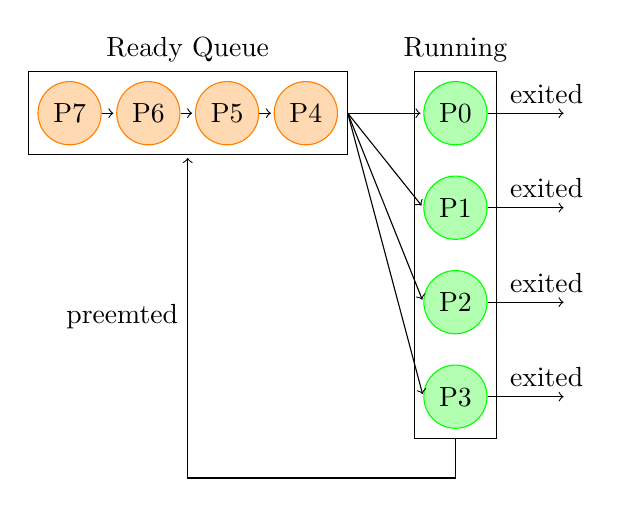
\begin{tikzpicture}[shorten >=1pt,node distance=1.0cm,on grid,auto,
				running/.style={circle, draw=green!100, fill=green!30},
				ready/.style={circle, draw=orange!100, fill=orange!30}
			]
			
			\node[ready] (p_4) [] {P4};
			\node[ready] (p_5) [left=of p_4] {P5};
			\node[ready] (p_6) [left=of p_5] {P6};
			\node[ready] (p_7) [left=of p_6] {P7};
			
			\node[state,rectangle] (q_0) [fit={(p_4) (p_5) (p_6) (p_7)}] [label=Ready Queue] {};
			
			\node[running] (r_0) [right=of q_0, xshift=24mm] {P0};
			\node[running] (r_1) [below=of r_0, yshift=-2mm] {P1};
			\node[running] (r_2) [below=of r_1, yshift=-2mm] {P2};
			\node[running] (r_3) [below=of r_2, yshift=-2mm] {P3};
			
			\node[state,rectangle] (q_1) [fit={(r_0) (r_1) (r_2) (r_3)}] [label=Running] {};
			
			\draw[->] (q_0.east) -- (r_0.west);
			\draw[->] (q_0.east) -- (r_1.west);
			\draw[->] (q_0.east) -- (r_2.west);
			\draw[->] (q_0.east) -- (r_3.west);
			
			\draw[->] (p_7.east) -- (p_6.west);
			\draw[->] (p_6.east) -- (p_5.west);
			\draw[->] (p_5.east) -- (p_4.west);
			
			\draw[->] (r_0.east) -- ++(10mm,0) node[near end] {exited};
			\draw[->] (r_1.east) -- ++(10mm,0) node[near end] {exited};
			\draw[->] (r_2.east) -- ++(10mm,0) node[near end] {exited};
			\draw[->] (r_3.east) -- ++(10mm,0) node[near end] {exited};
			     
			\draw[->] (q_1.south) |- ++(0,-5mm) -| (q_0.south) node[near end] {preemted};
		\end{tikzpicture}
		\caption{Global Ready Queue}
	\end{subfigure}
	% 
	\begin{subfigure}{.48\linewidth}
		\centering
		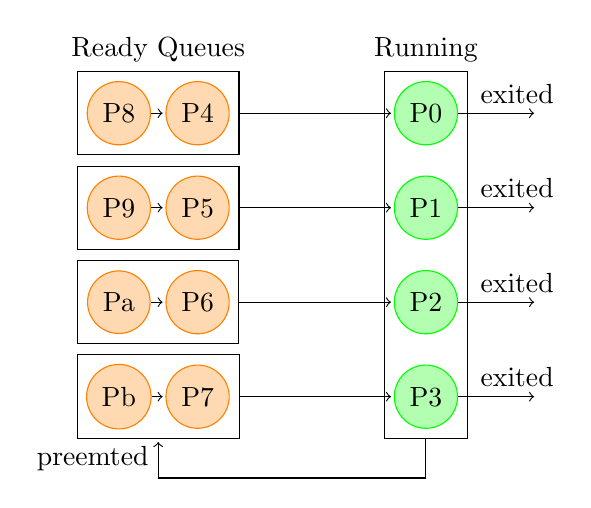
\begin{tikzpicture}[shorten >=1pt,node distance=1.0cm,on grid,auto,
				running/.style={circle, draw=green!100, fill=green!30},
				ready/.style={circle, draw=orange!100, fill=orange!30}
			]
			
			\node[ready] (p_4) [] {P4};
			\node[ready] (p_5) [below=of p_4, yshift=-2mm] {P5};
			\node[ready] (p_6) [below=of p_5, yshift=-2mm] {P6};
			\node[ready] (p_7) [below=of p_6, yshift=-2mm] {P7};
			
			\node[ready] (p_8) [left=of p_4] {P8};
			\node[ready] (p_9) [left=of p_5] {P9};
			\node[ready] (p_10) [left=of p_6] {Pa};
			\node[ready] (p_11) [left=of p_7] {Pb};    
			
			\node[state,rectangle] (q_0) [fit={(p_4) (p_8)}] [label=Ready Queues] {};
			\node[state,rectangle] (q_1) [fit={(p_5) (p_9)}] [below=of q_0, yshift=-2mm] {};
			\node[state,rectangle] (q_2) [fit={(p_6) (p_10)}] [below=of q_1, yshift=-2mm] {};
			\node[state,rectangle] (q_3) [fit={(p_7) (p_11)}] [below=of q_2, yshift=-2mm] {};
			
			\node[running] (r_0) [right=of q_0, xshift=24mm] {P0};
			\node[running] (r_1) [below=of r_0, yshift=-2mm] {P1};
			\node[running] (r_2) [below=of r_1, yshift=-2mm] {P2};
			\node[running] (r_3) [below=of r_2, yshift=-2mm] {P3};
			
			\node[state,rectangle] (q_r) [fit={(r_0) (r_1) (r_2) (r_3)}] [label=Running] {};
			
			\draw[->] (q_0.east) -- (r_0.west);
			\draw[->] (q_1.east) -- (r_1.west);
			\draw[->] (q_2.east) -- (r_2.west);
			\draw[->] (q_3.east) -- (r_3.west);
			
			\draw[->] (p_8.east) -- (p_4.west);
			\draw[->] (p_9.east) -- (p_5.west);
			\draw[->] (p_10.east) -- (p_6.west);
			\draw[->] (p_11.east) -- (p_7.west);
			     
			\draw[->] (q_r.south) |- ++(0,-5mm) -| (q_3.south) node[near end] {preemted};
			\draw[->] (r_0.east) -- ++(10mm,0) node[near end] {exited};
			\draw[->] (r_1.east) -- ++(10mm,0) node[near end] {exited};
			\draw[->] (r_2.east) -- ++(10mm,0) node[near end] {exited};
			\draw[->] (r_3.east) -- ++(10mm,0) node[near end] {exited};
		\end{tikzpicture}
		\caption{Core Ready Queue}
	\end{subfigure}
	\caption{Scheduler Structures}
\end{figure*}

% DONE
Under the current scheduler, a process, if eligible, is migrated during preemption.  In general, the scheduler will opt to keep a process on the same CPU unless another core is sufficiently empty or its affinity set dictates otherwise.  In essence, as processes are rescheduled, the cores will tend towards a balanced configuration.  However, it is also possible that a core will have a stream of processes terminate leading to a load imbalance between ready queues (fig. 3).
% DONE

\begin{figure}[!h]
	\centering
	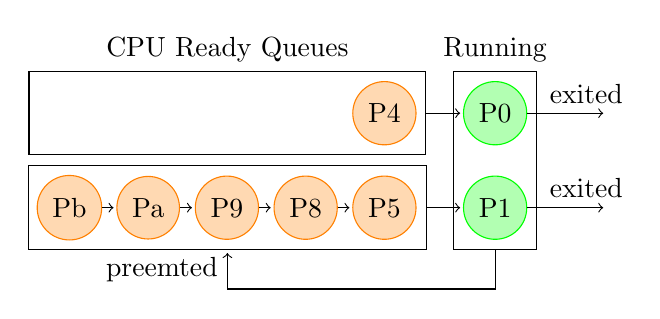
\begin{tikzpicture}[shorten >=1pt,node distance=1.0cm,on grid,auto,
			running/.style={circle, draw=green!100, fill=green!30},
			ready/.style={circle, draw=orange!100, fill=orange!30},
			empty/.style={circle, draw=none, fill=none, text=white}
		]
		
		\node[ready] (p_4) [] {P4};
		\node[ready] (p_5) [below=of p_4, yshift=-2mm] {P5};
		
		\node[ready] (p_6) [left=of p_5] {P8};
		\node[ready] (p_7) [left=of p_6] {P9};
		\node[ready] (p_8) [left=of p_7] {Pa};
		\node[ready] (p_9) [left=of p_8] {Pb}; 
		    
		\node[empty] (p_e) [above=of p_9, yshift=+2mm] {Pe};
		
		\node[state,rectangle] (q_0) [fit={(p_4) (p_e)}] [label=CPU Ready Queues] {};
		\node[state,rectangle] (q_1) [fit={(p_5) (p_6) (p_7) (p_8) (p_9)}] [below=of q_0, yshift=-2mm] {};
		
		\node[running] (r_0) [right=of q_0, xshift=24mm] {P0};
		\node[running] (r_1) [below=of r_0, yshift=-2mm] {P1};
		
		\node[state,rectangle] (q_r) [fit={(r_0) (r_1)}] [label=Running] {};
		
		\draw[->] (q_0.east) -- (r_0.west);
		\draw[->] (q_1.east) -- (r_1.west);
		
		\draw[->] (p_9.east) -- (p_8.west);
		\draw[->] (p_8.east) -- (p_7.west);
		\draw[->] (p_7.east) -- (p_6.west);
		\draw[->] (p_6.east) -- (p_5.west);
		     
		\draw[->] (q_r.south) |- ++(0,-5mm) -| (q_1.south) node[near end] {preemted};
		\draw[->] (r_0.east) -- ++(10mm,0) node[near end] {exited};
		\draw[->] (r_1.east) -- ++(10mm,0) node[near end] {exited};
	\end{tikzpicture}
	\caption{Unbalanced Scheduling}
\end{figure}

% DONE
\textbf{FIG}
Pull migration is an effort to improve the re-balancing latency for queues which exhibit the behavior in fig. 3.  Periodically, an idle core will search for an overloaded core and pull eligible processes from the tail of its queue.  This task requires locking the busy queue for a longer period of time; while, the idle queue tends to have its lock acquired more frequently.  This task leads to high lock contention for both queues which can negatively impact the time spent in the kernel.  Specifically, while iterating, the busy core will be unable to retrieve the next runnable process.  Thus, it is important to pick a large enough interval to do the re-balancing that it does not cause much strain on performance.  However, in most cases, if a core is not sufficiently loaded the pull migration task will instead exit prematurely instead of locking both cores.

With respect to fairness, there are several areas which should be discussed.  With the global queue, all processes are allocated the same timeslice and have no core preference to help distribute the cache load.  Effectively, this means that all process share the same level of execution fairness; however, with per-core runqueues, core queue imbalance leads to execution latency on busy queues compared to that of an idle queue.  Migration aims to reduce the latency due to imbalance; yet it introduces migration unfairness.  For example, migrating a process will lead to a full L1 cache reload on the new core.  Thus, the initial form of migration during preemption tends to be relatively unfair towards recently executed processes, because they are the most affected by a cache reload.  Since processes are migrated from the end of the queue, a process is guaranteed to execute sooner on the idle queue.  Additionally, processes at the end of a queue exhibit poor temporal locality relative to the rest of the queue; and hence the cache penalty on migration is minimized as a partial reload may be required by the time the process is scheduled.
% DONE

\section{Performance}
\label{sec:performance}
% DONE
Different user programs were tested against the variations of the OS scheduler described previously.  In general, the tests consist of performing a scalar multiply for a specified runtime.  These tests aim to simulate process cache access and utilization and provide repeatable results for user and kernel event counters.

Total runtime is also presented in clock ticks; yet, is generally inaccurate since it includes the I/O overhead when dumping metrics over \texttt{stdout}.  Additionally, all data comfortably fits into the L2 cache and; thus, pipeline stalls involved when fetching from main memory are limited to the initial cold start.
% DONE

To describe the behavior for execution some terms should be defined.
\begin{itemize}
	\item \textbf{Work}: size of data used by a \textbf{single} thread relative to a processors L1 data cache
	\begin{itemize}
		\item uint64\_t[20][25] 	= 25\% L1 data cache	= small matrix
		\item uint64\_t[40][50] 	= 100\% L1 data cache	= medium matrix
		\item uint64\_t[80][100] 	= 400\% L1 data cache	= large matrix
	\end{itemize}
	\item \textbf{Samples}: the global number of work entries available for execution by \textbf{all} threads
	\begin{itemize}
		\item 4 independent work entries 	= high spatial locality
		\item 16 independent work entries 	= low spatial locality
	\end{itemize}
	\item \textbf{Difficulty}: a relative measure of bounded execution time by a single thread
	\begin{itemize}
		\item $10^2$ repeated computations = easy
		\item $10^3$ repeated computations = normal
		\item $10^4$ repeated computations = hard
	\end{itemize}
\end{itemize}

\begin{figure*}[!h]
	\caption{single core baseline comparison}
	\centering
	\begin{subtable}{.48\linewidth}
		\centering
		\begin{tabular}{ l|rrr }
			Type    & Total     & User      & Kernel  \\
			\hline
			Instrs  & 467617788 & 466380022 & 1237766 \\ 
			Cycles  & 693267321 & 691411106 & 1856215 \\ 
			Access  & 264291472 & 263665636 & 625836  \\ 
			Refill  & 1539      & 1340      & 199     \\ 
			Runtime & 45374884  & -         & -       \\ 
			\hline
		\end{tabular}
		\caption{single core - matrix 1x utilization}
	\end{subtable}
	\hfill
	\begin{subtable}{.48\linewidth}
		\centering
		\begin{tabular}{ l|rrr }
			Type    & Total      & User       & Kernel  \\
			\hline
			Instrs  & 1858506765 & 1853566311 & 4940454 \\ 
			Cycles  & 2768987855 & 2760678046 & 8309809 \\ 
			Access  & 1050488228 & 1047990323 & 2497905 \\ 
			Refill  & 1389770    & 1293188    & 96582   \\ 
			Runtime & 178608294  & -          & -       \\ 
			\hline
		\end{tabular}
		\caption{single core - matrix 4x utilization}
	\end{subtable}
\end{figure*}

% DONE
The examples serve as baselines for comparing behaivour when scaling the problem to multiple cores.  The first example will operate on a small matrix, while the second uses a large matrix requiring a full cache refill on each iteration (with some degree of randomness relating to the replacement policy).  On the second data set, the results are predictably much larger due to frequent data thrashing.  However, despite a huge difference in APR, the total relative runtime seems to be fairly independent.  This is likely a side effect of the L1 automatic prefetcher which when a pattern is detected, will start linefills in the background \cite{arm-l1-prefetch}.  This prefetcher likely will cause skewed results for most of the computation since the tests have a very consistent access pattern.  Thus, in general, cache APR will have a higher impact especially from the schedulers perspective; where there is unlikely to be similar patterns between user processes.
% DONE

\begin{figure*}[!h]
	\caption{strided matrix multiplication running against different schedulers}		
	\centering
	\begin{subtable}{.48\linewidth}
		\centering
		\begin{tabular}{ l|rrr }
			Type    & Total     & User      & Kernel  \\
			\hline
            Instrs & 1316124843 & 1313462560 & 2662283 \\
            Cycles & 1960863928 & 1956137419 & 4726509 \\
            Access & 744181293 & 742708916 & 1472377 \\
            Refill & 537874 & 509212 & 28662 \\
            Runtime & 41175374 & - & - \\
			\hline
		\end{tabular}
		\caption{multi core - global queue}
	\end{subtable}
	\begin{subtable}{.48\linewidth} 
		\centering        
		\begin{tabular}{ l|rrr }
			Type    & Total     & User      & Kernel \\
			\hline
            Instrs & 1168350039 & 1164789764 & 3560275 \\
            Cycles & 1734415365 & 1728844371 & 5570994 \\
            Access & 660416972 & 658632902 & 1784070 \\
            Refill & 69361 & 47662 & 21699 \\
            Runtime & 40603738 & - & - \\
			\hline
		\end{tabular}
		\caption{multi core - cpu queue (affinity)}    
	\end{subtable}
\end{figure*}

% DONE
Extending the previous examples to a multicore system demonstrates the benefit of well thought out parallelization.  A large matrix is separated into four medium strided matrices and will execute at hard difficulty.  They will be executed against both the global scheduler and the core scheduler with fixed process affinity to separate computation onto each of the four cores.  Without comparing the differences between the two schedulers, they both outperform the single core computation on the same problem size.  Suprisingly, both exhibit superlinear speedup.

Likely, the biggest factor to this speedup is the result of data being precached in the L2 cache by the other processors.  As a result of striding, the innermost matrix edges will exhibit high spatial locality; while having low temporal locality.  This temporal locality effectively acts as a form of prefetching for subsequent accesses by other threads to the L2 cache.
% DONE

\textbf{TODO: Possibly mention kernel decrease in performance... this was suprising}

\begin{figure*}[!h]
	\caption{60 threads consisting of 48 hard processes and 12 easy processes}	
	\centering
	\begin{subtable}{.48\linewidth}
		\centering                 
		\begin{tabular}{l|rrr}
			Type    & Total      & User       & Kernel     \\
			\hline
			Instrs  & 1543135939 & 1396850683 & 146285256  \\ 
			Cycles  & 3146576481 & 2076522276 & 1070054205 \\ 
			Access  & 845516444  & 789349384  & 56167060   \\ 
			Refill  & 7653514    & 112360     & 7541154    \\ 
			Runtime & 152657484  & -          & -          \\
			\hline 
		\end{tabular}
		\caption{without pull migration (high locality)}
	\end{subtable}
	\hfill
	\begin{subtable}{.48\linewidth}
		\begin{tabular}{l|rrr}
			Type    & Total      & User       & Kernel    \\
			\hline
			Instrs  & 1468299596 & 1398454567 & 69845029  \\ 
			Cycles  & 2552848279 & 2079318879 & 473529400 \\ 
			Access  & 816022596  & 790256656  & 25765940  \\ 
			Refill  & 3126952    & 140213     & 2986739   \\ 
			Runtime & 156804356  & -          & -         \\
			\hline
		\end{tabular}
		\caption{with pull migration (high locality)}
	\end{subtable}
	\begin{subtable}{.48\textwidth}
		\centering                 
		\begin{tabular}{l|rrr}       
			Type    & Total      & User       & Kernel     \\
			\hline
			Instrs  & 1613944771 & 1404552990 & 209391781  \\ 
			Cycles  & 3491698429 & 2086636583 & 1405061846 \\ 
			Access  & 873214573  & 793699999  & 79514574   \\ 
			Refill  & 9792188    & 28820      & 9763368    \\ 
			Runtime & 152321428  & -          & -          \\ 
			\hline
		\end{tabular}
		\caption{without pull migration (low locality)}
	\end{subtable}
	\hfill
	\begin{subtable}{.48\textwidth}
		\centering                 
		\begin{tabular}{l|rrr}  
			Type    & Total      & User       & Kernel    \\
			\hline
			Instrs  & 1520575475 & 1445743126 & 74832349  \\ 
			Cycles  & 2574353547 & 2147872630 & 426480917 \\ 
			Access  & 843643737  & 816978128  & 26665609  \\ 
			Refill  & 2283806    & 34930      & 2248876   \\ 
			Runtime & 161631896  & -          & -         \\ 
			\hline
		\end{tabular}
		\caption{with pull migration (low locality)}        
	\end{subtable}
\end{figure*}

% DONE
To test the behavior of the system under a rapid stream of terminating processes difficulty was split into 12 hard threads and 60 easy threads designed to quickly terminate.  For each example, small matrices were tested under both cases for spatial locality.

The impact of pull migration is immediately evident in a 15-20\% cycle count and 25\% refill rate differentials with push migration.  Despite having apparent cache benefit, the significant improvement is in the kernel.  With pull migration, the total number of kernel instructions and cycles drops significantly.  This is likely related to decreased core lock contention.

When a core quickly empties, the remaining cores will attempt to push work onto that idle queue under normal scheduling.  Since all cores are competing for the idle cores lock, the cores effectively serialize themselves until they are balanced.  Since a full balancing may require several context switches this affect can be quite common.  However, with pull migration, instead of having many repeated requests to the idle core runqueue, a busy queue will offload work until both are balanced, hence decreasing the number of context switches and lock contention required to balance the queues.
% DONE

\begin{figure*}[!h]
	\caption{even distribution of easy, normal and hard threads}
	\centering
	\begin{subtable}[b]{.48\linewidth}
		\centering                 
		\begin{tabular}{ l|rrr }
			Type    & Total      & User       & Kernel    \\
			\hline
			Instrs  & 2945961318 & 2829092653 & 116868665 \\ 
			Cycles  & 4881259967 & 4206238780 & 675021187 \\ 
			Access  & 1642115209 & 1598721424 & 43393785  \\ 
			Refill  & 4570467    & 298213     & 4272254   \\ 
			Runtime & 175864992  & -          & -         \\
			\hline
		\end{tabular}
		\caption{without pull migration}    
	\end{subtable}
	\hfill
	\begin{subtable}[b]{.48\linewidth}
		\centering
		\begin{tabular}{ l|rrr }
			Type    & Total      & User       & Kernel    \\
			\hline
			Instrs  & 2727027846 & 2625810066 & 101217780 \\ 
			Cycles  & 4421745433 & 3903078399 & 518667034 \\ 
			Access  & 1520521397 & 1483845439 & 36675958  \\ 
			Refill  & 3226996    & 222090     & 3004906   \\ 
			Runtime & 171909144  & -          & -         \\
			\hline
		\end{tabular}
		\caption{with pull migration}
	\end{subtable}
\end{figure*}

% DONE
While the previous example demonstrated the short-term benefit of pull migration, this case utilizes an even distribution of difficulty operating on a small matrix with low spatial locality between threads to demonstrate long-term scheduling benefits.  Processes at the end of a runqueue will exhibit poor temporal locality and hence are less likely to have valid cache data by the time they run.  Thus, moving a process from the tail of a runqueue will end up minimizing the migration penalty of moving a recently executed process.  In this case, when a group of processes dies, the cache space that they used can now be evenly distributed across fewer processes resulting in better utilization while decreasing thrashing.  This decrease in cache pollution enables more work per time slice and leads to fewer context switches; thus, resulting in quicker execution time.
% DONE

\begin{figure*}[!h]
	\caption{comparison between thread pool and fully threaded execution}
	\centering
	\begin{subtable}{.48\textwidth}
		\centering
		\begin{tabular}{ l|rrr }
			Type    & Total      & User       & Kernel    \\
			\hline
			Instrs & 858992530 & 753437017 & 105555513 \\ 
			Cycles & 1910983635 & 1123087469 & 787896166 \\ 
			Access & 465293588 & 426171724 & 39121864 \\ 
			Refill & 5513845 & 210562 & 5303283 \\ 
			Runtime & 165487634 & - & - \\ 
			\hline
		\end{tabular}
		\caption{threads (high locality)}
	\end{subtable}
	\hfill
	\begin{subtable}{.48\textwidth} 
		\centering
		\begin{tabular}{ l|rrr }
			Type    & Total      & User       & Kernel    \\
			\hline
			Instrs & 825909448 & 773161950 & 52747498 \\ 
			Cycles & 1462457892 & 1162415850 & 300042042 \\ 
			Access & 453475978 & 435856372 & 17619606 \\ 
			Refill & 1737886 & 364441 & 1373445 \\ 
			Runtime & 61557018 & - & - \\
			\hline
		\end{tabular}
		\caption{pooled (high locality)}        
	\end{subtable}
\end{figure*}

\begin{figure*}[!h]
	\begin{subtable}{.48\textwidth} 
		\centering
		\begin{tabular}{ l|rrr }
			Type    & Total      & User       & Kernel    \\
			\hline
			Instrs & 850652290 & 757440549 & 93211741 \\ 
			Cycles & 1900834361 & 1127333154 & 773501207 \\ 
			Access & 463377065 & 428435448 & 34941617 \\ 
			Refill & 5282763 & 128873 & 5153890 \\ 
			Runtime & 165916644 & - & - \\
			\hline
		\end{tabular}
		\caption{threads (low locality)}
	\end{subtable}
	\hfill
	\begin{subtable}{.48\textwidth} 
		\centering
		\begin{tabular}{ l|rrr }
			Type    & Total      & User       & Kernel    \\
			\hline
			Instrs & 819945002 & 764500953 & 55444049 \\ 
			Cycles & 1522878029 & 1144994038 & 377883991 \\ 
			Access & 450320681 & 431461874 & 18858807 \\ 
			Refill & 2026635 & 131657 & 1894978 \\ 
			Runtime & 61636292 & - & - \\
			\hline
		\end{tabular}
		\caption{pooled (low locality)}
	\end{subtable}
\end{figure*}

% DONE
In Fig. 7, 64 threads operating on a small matrix are scheduled into independent threads assigned work \textbf{or} 16 worker threads pulling work from a protected queue.  They run under the same difficulty; however, locality between the two classes of samples is evaluated separately.

For these examples, the primary difference is evident in the thrashing in the kernel.  As more processes become preempted, the total amount of active memory increases leading to full cache utilization by user processes.  In general, this leads to eviction of kernel cache lines; resulting in a 20-30\% increase in kernel IPC.  However, pooling does result in poorer performance with regards to shared memory.  Since the active subset of work is much more constrained, two processes which may be working on the same subset of data are unlikely to be scheduled on the same core.  When there is relatively low locality between workers, the difference between single threaded and pooled is minimal; however, with high locality, pooling results in a 40\% reduction in APR.
% DONE

\section{Conclusion}
\label{sec:conclusion}

Conclusions here \cite{freebsd} \cite{unix}.
\textbf{TODO: talk about the L2 cache in conclusion as it amplifies performance penalty}

At the core of most systems, an OS facilitates process execution with synchronization primitives and multiprocessing.  Compared to a cooperative OS, a preemptive OS presents additional challenges relating to scheduling and cache performance.  In general, since a process may be preempted at any point during execution it can be difficult to reason about performance in a local context.  From a global context, a preemptive system will incur additional costs relating to the frequency of context switching and cache pollution when not dealing with shared memory.  The scheduler plays an important role in determining execution order and CPU binding to minimize this overhead.  In SMP systems, the general goal to balance execution across cores tends to be a good approach.  However, it does not address the costs related to preemption.  Primarily naive balancing will tend to over-pollute cores; thus, more robust approaches involving CPU binding can help minimize this.  Yet, CPU affinity easily reintroduces the problem of unbalanced processors.

To maintain the benefit of CPU binding while attempting to keep computation balanced, process migration plays an important role.  A short-term and long-term load balancer provide different benefits to global performance.  The short-term load balancer, ensures that work is consistently evenly distributed across cores; however, it suffers performance penalties when migrating many processes.  Specifically there tends to be a high cache penalty when migrating processes with the short-term scheduler.  For long-term load balancing, pull migration tends to migrate tasks which have a lower cache penalty.

% These migration policies generally work well for the simplification that 

It is important to note that for all tests, despite having a cache penalty; much was offset by the ARM prefetch module and all data fitting in the L2 data cache.  This is important since other programs may not be easily classified by the prefetch module and in larger systems there is often a larger cache penalty since data is less likely to be cached in the L2 cache.

\section{Lessons Learned}
\label{sec:lessons}
Since the development of the operating system was done from the ground up there were plenty of learning opportunities along the way. 
\textbf{TODO} 

Measuring success in a bare metal environment can prove to be quite difficult; thus, it became important to progressively escalate to better debugging utilities.  Initially, bare minimum assembly required to toggle an LED gave limited success or failure output.  The jump to FTDI was helpful in debugging simple conditions and CPU registers.  Finally, for tracing complex execution; having a proper debugging protocol with JLink, OpenOCD and GDB enabled better debugging for context switching, exception handling and multicore execution.

The initial JLink setup proved to be quite tricky due to incompatibility with the current version of OpenOCD, mismatched toolchain and microcontroller architecture/configuration.  However, the end result was incredibly important to establishing a successful development workflow.  Instead of having to perform a careful SD card dance between my computer and the Pi, having the capability to flash to RAM allowed for much quicker development cycles.  Initially, I had looked into alternative bootloaders (UBoot, GRUB) which can work over ethernet or serial connections; however, in general the end result of having proper host debugging utilities was invaluable.

On the topic of toolchain incompatibility, code was initially compiled using \texttt{arm-none-eabi} which is used for cross compiling to 32-bit ARM and while aarch64 offers compatibility with older architecture, the generic debug interface is much less compatible.  Thus, it is important to recognize that despite older systems often having more documentation; the complexity of developing on a compatibility layer is not worth the extra effort.  Additionally, the aarch64 architecture proved to have clear and better structured semantics especially related to exception handling.  The exception model for aarch64 is standardized across four types; whereas, the ARMv7-A architecture had various subsets of banked registers and return instructions dependent on the interrupt source.  Additionally, the addition of a unified exception status register (ESR) was much more helpful with determining the cause of a processor fault.

Newlib was designed to provide the C library on embedded systems \cite{newlib} with minimal system support handled by low level functions.  For example, the overhead of implementing the \texttt{malloc} and \texttt{printf} routines was reduced to simply stubbing out \texttt{sbrk} and establishing a minimal device descriptor table for \texttt{stdout}.  As I built the system with the design of having POSIX compliancy, I additionally included the \texttt{<sys>} headers from Newlib; which often imposed lower level structure restrictions.  For example, when implementing CPU sets I wanted to follow the same type of implementation as embedding the affinity set in the \texttt{pthread\_attr\_t} which was hidden around several macro guards; which when enabled led to conflicts in other areas.  Thus, for long-term kernel development; having custom POSIX headers is beneficial to customizability of the system and allows the system to not be constrained by ``immutable'' or \textbf{static} headers.

\section{Future Work}
\label{sec:future}
- exception higherarchy from EL0 up to EL1

- better POSIX compliancy thus port more complex programs to run tests against.
eg. real programs; what would the necessary components be?, networked bounded programs, file bounded programs

- device drivers in multicore domain, network drivers would likely be interesting to explore.  also sockets and their implementation

- user virtual address space and compare the performance penalty for TLB reloads

- slab allocation algorithms for a more complex system

- implementation of the linux rb-tree scheduler with implications for migration, variable quantum size + penalizing bad programs

- better migration policies with book-keeping.

- microkernel architecture + performance

- run to idle then pull, with idle sleeping

% \section{Acknowledgements} 

\onecolumn
\begin{sloppypar}
	\bibliographystyle{acm}
	\bibliography{biblio}
\end{sloppypar}

% \end{multicols}
\end{document}